\chapter{Introduction}
\section{The language and its speakers}\label{sec:1.1}

Pichi is an Afro-Caribbean English-lexifier Creole language (Ethnologue code “fpe”) spoken on the island of Bioko, Equatorial Guinea (cf. \figref{map:1:1.1}). Pichi is the most widely spoken language of the country’s capital Malabo next to \ili{Spanish}, and it serves as a primary language to a large proportion of the capital’s inhabitants. Pichi is also used as a primary language in a number of villages and towns along the Coast of Bioko, amongst them Sampaca, Fiston, Basupú, Barrio Las Palmas, and Luba (Morgades Besari, p.c.), and it is spoken as a lingua franca throughout Bioko (cf. \figref{map:1:1.2} below). The language is also used by a sizeable community of people originating from Bioko in Bata, the largest town on the continental part of the country. In the literature, Pichi is known under the names “Fernando Po Creole English” \citep{SimonsFennig2017}, “Fernando Po Krio” \citep{Berry1970},  “Fernandino Creole English” \citep{Holm1988}, “Pidgin (English)” (Morgades Besari, p.c.) “Broken English” \citep{Zarco1938}, and “Pichinglis” \citep{Lipski1992}. While older speakers sometimes refer to the language as “Krio” or “Pidgin”, most present-day speakers refer to it as “Pichinglis”, “Pichin” with a nasalised final vowel, or “Pichi” \textit{tout court}. 

Pichi descends from 19\textsuperscript{th} century \ili{Krio}, which first arrived in Bioko, the former Fernando Po, with African settlers from Freetown, Sierra Leone, in 1827 \citep[165]{Fyfe1962}. \ili{Krio}, in turn, emerged as the principal language of the urban population of Freetown, Sierra Leone, from the late 18\textsuperscript{th} century onwards \citep{Huber1999}. Modern Krio\il{Krio} and Pichi are therefore both descendants of Early Krio. Linguistic and historical evidence suggests that the diffusion of \ili{Krio} along the west coast of Africa in the 19\textsuperscript{th} century also contributed significantly to the formation of Nigerian Pidgin, Cameroon Pidgin, and Ghanaian Pidgin English \citep{Huber1999}. 

No linguistic census data exist in Equatorial Guinea, but probably up to 70 per cent of the population of Bioko island, hence well above 100,000 speakers, regularly use Pichi at various levels of nativisation and in various multilingual and multilectal constellations in and outside their homes \citep[194]{Yakpo2013}. Next to Pichi, at least fourteen languages are spoken by the peoples of Equatorial Guinea \citep{Hammarstrom2017}. \ili{Fang} has the largest number of speakers, but its use is largely limited to the continental part of the country (also referred to as “Río Muni”\textstyleannotationreference{)}. \ili{Bubi} is probably the second most widely spoken African language of the country, but its use is, in turn, limited to Bioko. There is an established pattern of language shift to Pichi and \ili{Spanish} in Malabo and other larger agglomerations of Bioko, and there are indications that Bubi is under increasing pressure from these two languages. Equatorial Guinea also harbours the Portuguese-lexifier creole Fa d’Ambô, spoken by the people of the island of Annobón (cf. \figref{map:1:1.1}). Fa d’Ambô shares historical and linguistic ties with the other Portuguese-lexifier creoles of the Gulf of Guinea, namely Lungwa Santome and Lunga Ngola (Angolar) in São Tomé, and Lung’Ie in Príncipe \citep{Post2013}. 

Mutual intelligibility between Pichi, \ili{Krio}, Cameroon Pidgin, Nigerian Pidgin, and Ghanaian Pidgin English is relatively high. However, an impediment to fluid communication between speakers of Pichi and its African sister languages is the divergent path of development of Pichi since 1857. In that year, Spain began to actively enforce colonial rule in Equatorial Guinea. From then onwards, Pichi was cut off from the direct influence of English. Pichi has therefore escaped the phonological, grammatical, and lexical convergence with English that has been documented for English-lexifier creoles spoken alongside \ili{English} (see e.g. \citealt{SalaNgefac2006} for Cameroon Pidgin). At the same time, Pichi has been in intense contact with \ili{Spanish} for over a century and has undergone substantial lexical and some structural influence from the colonial language of Equatorial Guinea . 

Equatorial Guinea has three \textit{de} \textit{jure} official languages, namely \ili{Spanish}, \ili{French}, and \ili{Portuguese}. From the primary to the tertiary levels, instruction is given alone in \ili{Spanish}, which is therefore the only \textit{de} \textit{facto} official language of the country. There is no legally or politically defined role for education in African languages (\citealt{Yakpo2011,Yakpo2016estatuto}). However, the national education bill currently in vigour (\citealt{RepublicadeGuineaEcuatorial2007}) offers the optional use of indigenous languages in education (\citealt{OloFernandes2012}). The socio-linguistic status of Pichi is particularly unfavourable among the natively spoken languages of Equatorial Guinea. During colonial rule, Pichi was considered an impoverished, debased form of \ili{English} by Spanish colonial administrators and missionaries (see \citealt[5–7]{Zarco1938} for a pungent exposition of this view). Pichi, like the other creole languages of the Atlantic Basin, still has to struggle with this difficult legacy. In spite of its great importance as a community language and as a national and regional lingua franca, Pichi enjoys no official recognition nor support, is conspicuously absent from public discourse and the official media, and until today, has no place in the educational policy of Equatorial Guinea \citep{Yakpo2016estatuto}.

\begin{figure}
	\caption{Map 1 Continental and insular Equatorial Guinea (in bold)}
	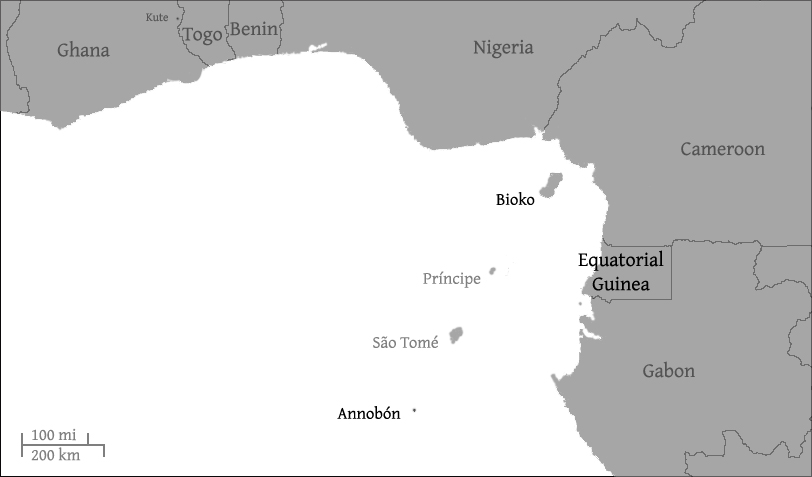
\includegraphics[width=\textwidth]{figures/yakpomod-img1.png}
	\label{map:1:1.1}
\end{figure}

\begin{figure}
	\caption{Map 2 Towns with Pichi-speaking communities in Bioko (in bold)}
	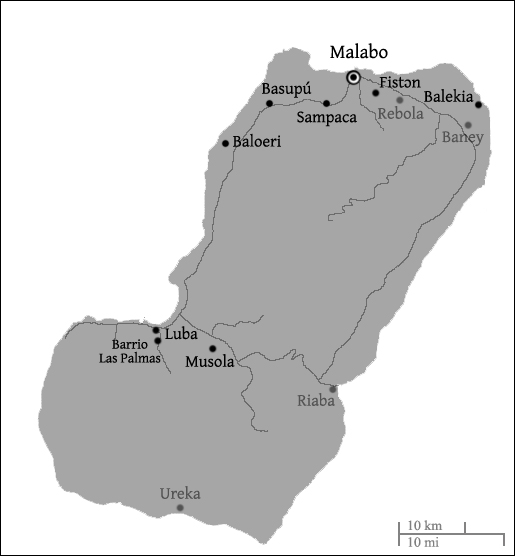
\includegraphics[width=.5\textwidth]{figures/yakpomod-img2.png}
	\label{map:1:1.2}
\end{figure}

The lingering colonialist perspective on Pichi and its sister languages in West Africa and across the Atlantic stands in stark contrast to the fact that these languages epitomise the achievements of African and African-descended peoples who, in resisting and adapting to the ignominious system of European slavery and colonialism, carved out in Africa and the Americas one of the largest, and today most vibrant cultural and linguistic zones of the world.

\section{Contact with Spanish}\label{sec:1.2}

\ili{Spanish} has left a deep imprint on the lexicon and grammar of Pichi. Codemixing is an integral part of the linguistic system of Pichi \citep{Yakpo2009complexity,Yakpo2018}. The pervasive influence of \ili{Spanish} on Pichi is for one part the consequence of language policy. Since colonial rule and the independence of Equatorial Guinea in 1968, Spanish has remained the sole medium of instruction at all levels of the educational system (\citealt[35–36]{Lipski1992}). There is a widespread competence in different registers of \ili{Spanish} by Pichi speakers in Malabo and Equatorial Guinea as a whole \citep{Lipski1985,García2016}. In Malabo, the acquisition of Spanish begins in early childhood, even for many working-class Equatoguineans with little or no school education. 

Another factor favouring codemixing is the positive attitude towards multilingualism in a highly polyglot society, against the background of a tenacious vitality of Pichi as a symbol of social identity. Presumably, Pichi-Spanish codemixing has for a long time served as a badge of identity for the population of Bioko in the course of a long history of immigration by speakers of other varieties of West African English-lexicon Creoles. Today, the language also plays an important role for the self-identification of those who grew up on the island in the face of an accelerated pace of internal migration by Equatoguineans from the mainland. \textit{Bɔ́n} \textit{na} \textit{yá,} \textit{gró} \textit{na} \textit{yá} ‘born here, grown up here’ is the mark which distinguishes Pichi-speaking islanders, irrespective of their ethnic background, from the late arrivals of mainland origin who speak little or no Pichi. 

Equally, the burgeoning oil economy of Equatorial Guinea has led to increased urbanisation, extending multi-ethnic social networks and the spread of Pichi as a native language. In such a socio-economic environment and amidst a high general competence in the official language Spanish, codemixing between Pichi and Spanish, rather than being exceptional, is consciously and confidently articulated in daily life (cf. chapter 11 for a detailed description of codemixing). Pichi is also in contact with other African languages spoken in the region, amongst them Fang and Bubi, as well as Nigerian and Cameroonian Pidgin (\citealt{Yakpo2013} discusses influences on Pichi from these languages).

\section{Variation}\label{sec:1.3}

The variation recorded in Pichi appears to be determined by a mixture of the factors age, language background, and social class. Phonological variation is particularly conspicuous. Some of the variation in Pichi may be captured by an albeit oversimplified division of speakers into two groups. Group 1 principally consists of the Fernandinos, the old commercial and social elite of Bioko \citep{Lynn1984} that inhabits the historical centre of Malabo and has used Pichi as a home language since the 19\textsuperscript{th} century. Group 1 also comprises people of diverse ethno-linguistic backgrounds who grew up in Malabo in the ambit of Fernandino culture. The lexicon, grammar, and phonology of Group 1 reflects an earlier chronolect of Pichi, which is also closer to (early) Krio. 

Group 2 is larger and culturally more diverse by incorporating “nuevos criollos” (Morgades Besari, p.c.) who have been accultured more recently into the Pichi-speaking urban culture of Malabo. It encompasses a large number of speakers with a Bubi cultural background who have shifted to Pichi as a primary language \citep{BolekiaBoleká2007}, and it includes large numbers of speakers with varying degrees of nativisation. Group 1 is shrinking at the expense of Group 2 through rapid urbanisation, immigration, and language shift. The terms “Mesopidgin” and “Acropidgin” employed by \citet{MorgadesBesari2011} capture some of the socio-linguistic differences between Group 1 and Group 2. The distinction between Group 1 and 2 is also reflected in apparent-time differences, where older speakers (principally those who came of age in the colonial era and the first decade of independence) tend to use the Group 1 lect, and the young majority population of Malabo and Bioko tends to use the Group 2 lect. 

In this work, I privilege the description of the language of Group 2 in the wish to represent how Pichi is spoken by the young and multi-ethnic majority in the homes and streets of Malabo today. I nevertheless account for variation by employing alternate forms where they exist (e.g. \textit{nɔ́bà{\textasciitilde}nɛ́a} ‘\textsc{neg.prf}’, \textit{tínap{\textasciitilde}tánap} ‘stand (up)’), and some of them may reflect differences between Groups 1 and 2. In the following, I present a few generalisations of the variation present in my corpus. 

For Group 2 speakers, there is no phonemic contrast between the alveolar fricative [s] and the postalveolar fricative [ʃ] (\hyperref[ex:0.1]{1}), and this is systematically applied to all words where Group 1 speakers use [ʃ] (\hyperref[ex:0.2]{2}). Group 2 speakers also insert a palatal glide [j] between [s] and a following mid vowel where Group 1 uses [ʃ] alone (\hyperref[ex:0.3]{3}--\hyperref[ex:0.4]{4}):



% beginning of manual numbering of examples till (10)


\bigskip
\noindent\begin{tabularx}{\textwidth}{l llX lX}
% \lsptoprule
 &  & Group 1 &  & Group 2 & \\
% \midrule
(1) \label{ex:0.1}
         & \itshape so & \itshape \textup{[só]} & \itshape \textup{‘sew, so’} & \itshape \textup{[só]}  & ‘sew, show, so’\\
&  & \itshape \textup{[ʃó]}  & \itshape \textup{‘show’} &  & \\
(2) \label{ex:0.2}
         & \itshape fínis & \itshape \textup{[fínìʃ]} & \itshape \textup{‘finish’} & \itshape \textup{[fínìs]} & ‘finish’\\
(3) \label{ex:0.3}
         & \itshape sɔ́p & \itshape \textup{[ʃɔ́p]} & \itshape \textup{‘shop’} & \itshape \textup{[sjɔ́p]} & ‘shop’\\
(4) \label{ex:0.4}
         & \itshape nésɔn & \itshape \textup{[néʃɔ̀n]} & \itshape \textup{‘nation’} & \itshape \textup{[nésjɔ̀n]} & ‘nation’\\
% \lspbottomrule
\end{tabularx}

\bigskip
Group 2 speakers tend to neutralise the phonemic distinction between close-mid and open-mid vowels (\hyperref[ex:0.5]{5}–\hyperref[ex:0.6]{6}):

\bigskip
\noindent\begin{tabularx}{\textwidth}{l lX lX}
 &  & Group 1 & Group 2 & \\
% \lsptoprule
(5) \label{ex:0.5}
         & \itshape fɔ & [fò {\textasciitilde} fɔ̀] & [fɔ̀] & ‘\textsc{prep}’\\
& \itshape mɔ́ & [mó {\textasciitilde} mɔ́] & [mɔ́] & ‘more’\\
(6) \label{ex:0.6}
         & \itshape mék & [mék {\textasciitilde} mɛ́k] & [mék] & ‘make, \textsc{sbjv}’\\
& \itshape lɛk & [lèk {\textasciitilde} lɛ̀k] & [lɛ̀k] & ‘like (preposition)’\\
% \lspbottomrule
\end{tabularx}

\bigskip
Group 2 speakers also tend to nasalise [i]-final words with an H.L tonal configuration (\hyperref[ex:0.7]{7}) and to prenasalise [j]-initial words as in (\hyperref[ex:0.8]{8}). This may lead to the formation of homophones like (\hyperref[ex:0.9]{9}) and (\hyperref[ex:0.10]{10}) for Group 2 speakers:

\bigskip
\noindent\begin{tabularx}{\textwidth}{l ll lX}
 &  & Group 1 & Group 2 & \\
% \lsptoprule
(7) \label{ex:0.7}
         & \itshape lɔ́ki & [lɔ́kìn] & [lɔ́kì] & ‘be lucky’\\
& \itshape tɔ́sti & [tɔ́stìn] & [tɔ́stì] & ‘be thirsty’\\
(8) \label{ex:0.8}
         & \itshape yandá & [njàndá] & [jàndá] & ‘yonder’\\
(9) \label{ex:0.9}
         & \itshape yús & [njús] & [jús] & ‘use’\\
(10) \label{ex:0.10}
         & \itshape nyús & [njús] & [njús] & ‘news’\\
% \lspbottomrule
\end{tabularx}



% end of manual numbering of examples
\addtocounter{equation}{10}

\bigskip
There is also some variation in the use and acceptance of certain grammatical structures. For example, Group 2 speakers seem to prefer the negative perfect marker \textit{nɛ́a} over \textit{nɔ́ba}. Equally, a serial verb construction\is{serial verb constructions} (SVC) featuring the verb \textit{sté} ‘be long time’ is not readily accepted as grammatical by many Group 1 speakers (cf. \sectref{sec:11.2.5}) and may therefore be a more recent development. Conversely, other types of SVCs are more common with Group 1 than with Group 2. Amongst them are SVCs involving the verb \textit{ték} ‘take’ (cf. \sectref{sec:11.2.3}) and motion-direction SVCs involving the verbs \textit{gó} ‘go’ and \textit{kán} ‘come’ (cf. \sectref{sec:11.2.1}). \textit{Ték}-serialisation is very common in modern \ili{Krio} and all other African English-lexifier creoles. Group 2 speakers instead tend to employ a combination of a verb and a prepositional phrase in these contexts. A final area characterised by variation is the extent of Pichi-Spanish language contact. For example, the names of weekdays and numerals are almost exclusively expressed in Spanish by Group 2 speakers. Group 1 speakers have access to both English- and Spanish-derived lexicon. They may employ \textit{lunes} ‘Monday’ in a codemixed sentence, but are equally likely to use \textit{mɔ́nde} ‘Monday’. Further, English-derived numbers above five are rarely used by Group 2 speakers (cf. \sectref{sec:13.3.1}). In contrast, Group 1 speakers master a wider range of the Pichi numeral system. However, even with this group, Pichi numbers above ten are seldom heard.

\section{Affiliation}\label{sec:1.4}

Pichi belongs to the grouping of languages referred to in the literature by various appelations, among them “English-based Afro-American” \citep{Alleyne1980}, “Atlantic Anglophone Creoles” \citep{Hancock1986,Hancock1987} “Atlantic English-based Creoles” (e.g. \citealt{MuyskenSmith1990}), “Atlantic English Creoles” (e.g. \citealt{Baker1999}). In this work and others, I employ the term “Afro-Caribbean English-lexifier Creoles” (abbreviated AECs) \citep{Faraclas2004} as a label that includes information about the speaker population (\mbox{“Afro-”}, i.e. people of African ancestry) and the two world regions where the languages are mainly spoken (“Afro-Caribbean”, i.e. Africa and the Caribbean). The use of “lexifier” underscores the dynamic character of the \ili{English} input to the lexicon, which varies in size and nature between the different languages. 


All Afro-Caribbean English-lexifier Creoles are transmitted and learned in various ways within the family and serve as means of communication and identification to linguistic communities. I therefore dispense with the term “pidgin” with its socio-structural connations and use “creole” alone. When referring to the linguistic grouping, “Creole” is written with an initial capital letter. The generic term is written “creole” in lower case. 

With well over 100 million speakers, the Afro-Caribbean English-lexifier Creoles and Pidgin-Creoles (henceforth AECs) spoken in Africa and the Americas together constitute one of the largest lectal continua of the Western hemisphere in speaker numbers and geographical extent \citep[22–23]{Yakpo2016estatuto}. Besides Pichi, the African sub-grouping of the AECs contains \ili{Krio} (Sierra Leone), \ili{Aku} (Gambia), Ghanaian Pidgin English, Nigerian Pidgin, and Cameroonian Pidgin \citep{HuberGörlach1996,Huber1999,BakerHuber2001}. There are also historical connections and cross-influences with varieties of Liberian English \citep{Singler1997}. Even if many details are still unclear, the evidence that there is a degree of common ancestry between the African and Caribbean AECs is compelling (e.g. \citealt{Hancock1986,Hancock1987,Smith1987,Smith2015}). There are also indications of a historical relation of the AECs with African American English(es) \citep{Dillard1973,Rickford1999,Winford2017}.

Within the African AECs, Pichi is most directly related to the \ili{Krio} language of Sierra Leone. A comparison of the two languages yields systematic lexical and structural correspondences. But it also reveals some differences. To begin with, both languages share a large percentage of non-basic vocabulary\is{basic vocabulary}, as shown in (\ref{ex:1:7}a), with the same tonal configurations. However, the Yoruba (b), Mende (c), and Temne (d) component of the Pichi lexicon appears to be much smaller than that of Krio and is limited to a few words in the corpus (data from \citealt{FyleJones1980}):

\eabox{\label{ex:1:7}
\begin{tabularx}{\textwidth}{rllX}
   & Pichi & Krio & Gloss\\
a. & \itshape à & \itshape à & ‘I’\\
& \itshape pɔ́sin & \itshape pɔ́sin & ‘person’\\
& \itshape (s)tík & \itshape (s)tík & ‘tree’\\
& \itshape yáy & \itshape yáy & ‘eye’\\
& \itshape yés & \itshape yés & ‘ear’\\
& \itshape bɔbí & \itshape bɔbí & ‘breast’\\
& \itshape bɛlɛ́ & \itshape bɛlɛ́ & ‘belly, foetus’\\
& \itshape watá, wɔtá & \itshape watá, wɔtá & ‘water’\\
& \itshape dɔtí & \itshape dɔtí & ‘be dirty’\\
& \itshape fɔdɔ́n & \itshape fɔdɔ́m & ‘fall’\\
& \itshape chɔ́p & \itshape chɔ́p, ít & ‘eat’\\
& \itshape hós & \itshape hós & ‘house’\\
& \itshape tití & \itshape tití & ‘girl’\\
& \itshape mákit & \itshape mákit, mákɛt & ‘market’\\
& \itshape wɔwɔ́ & \itshape wɔwɔ́ & ‘be messed up, ugly’\\
& \itshape bɔkú & \itshape bɔkú & ‘be much’\\
& \itshape yangá & \itshape nyangá & ‘be ostentatious’\\
& \itshape dúya & \itshape dúya & ‘please’\\
b. & \itshape ógi & \itshape ógi & ‘corn porridge’\\
& \itshape kúsɛ́ & \itshape kúshɛ́ & ‘expression of empathy’\\
& \itshape {}--- & \itshape órewá & ‘goodbye greeting’\\
c. & \itshape nyɔ́ní & \itshape nyɔ́ní & ‘red ant’\\
& \itshape blɔkɔ́s & \itshape blɔkɔ́s & ‘scrotum, penis’\\
& \itshape kandá & \itshape kandá & ‘skin, bark’\\
d. & \itshape yabaś & \itshape yabás & ‘onion’\\
& \itshape {}--- & \itshape kunkubé & ‘kind of boat’\\
\end{tabularx}
}
The two languages also share a number of lexical items common to numerous African and American English-lexicon Creoles. These were first compiled by (\citealt{Smith1987,Smith2001,Smith2015}) and termed “Ingredient X, Y, and Z”. In \REF{ex:1:8}, I list all the relevant words contained in the Pichi corpus. They comprise “Ingredient X” words of African origin (a), “Ingredient Y” words of Portuguese origin (b), “Ingredient Z” words of English origin (c), as well as a few function words of diverse origin (d):

\eabox{\label{ex:1:8}
\begin{tabularx}{.9\textwidth}{rll}
         & Ingredient X, Y, Z & Gloss\\
a. & \itshape sósó & ‘only’\\
& \itshape pɔtɔpɔ́tɔ́ & ‘mud(dy) substance’\\
& \itshape akará & ‘bean cake’\\
& \itshape fufú & ‘fufu’\\
b. & \itshape sabí & ‘know’\\
& \itshape pikín & ‘child’\\
c. & \itshape kéch & ‘catch’\\
& \itshape yɛ́r(i) & ‘hear’\\
& \itshape ɛf(ɛ) & ‘if’\\
& \itshape bwɛ́l & ‘boil’\\
& \itshape (s)pwɛ́l & ‘spoil, spend’\\
d. & \itshape na & ‘\textsc{foc}’\\
& \itshape una, unu & ‘\textsc{2pl}’\\
& \itshape mék & ‘imperative\is{imperatives}, \textsc{sbjv}’\\
& \itshape de & ‘\textsc{ipfv}’\\
& \itshape dé & ‘there’\\
& \itshape dé & \textsc{‘be.loc’}\\
\end{tabularx}
}
Some of the differences in vocabulary between the two languages owe to the same phonological characteristics that differentiate the members of Group 1 (Pichi) and Group 2 (\ili{Krio}) in the preceding section. Hence, most speakers of Pichi make no phonemic distinction between alveolar and postalveolar fricatives (\ref{ex:1:9}a); the phonemic distinction between close-mid and open-mid vowels is neutralised by most speakers (b). 

In addition, the distinction between velar and labial nasal consonants tends to collapse in word-final position (c); phonological processes create preferred CV sequences (d), voiced obstruents are normally devoiced in word-final position (e), while other words have different coda consonants (f). In general terms, present-day Pichi as spoken by the majority of its speakers exhibits a tendency towards the reduction of phonemic contrasts when compared to Krio.

\eabox{\label{ex:1:9}
\begin{tabularx}{\textwidth}{r ll ll ll}
 & \multicolumn{2}{l}{Pichi} & \multicolumn{2}{l}{Krio} & Gloss\\
a. & \itshape sút & [sút] & \itshape shút & [ʃút] & ‘shoot’\\
b. & \itshape fɔ & [fɔ̀{\textasciitilde}fò] & \itshape fɔ & [fɔ̀] & ‘\textsc{prep}’\\
c. & \itshape frɔn & [frɔ̀n {\textasciitilde} frɔ̀m] & \itshape frɔm & [frɔ̀m] & ‘from’\\
d. & \itshape smɔ́l & [sìmɔ́ {\textasciitilde} sùmɔ́] & \itshape smɔ́l & [smɔ́l] & ‘be small’\\
e. & \itshape bíg & [bík] & \itshape bíg & [bíg] & ‘be big’\\
f. & \itshape (s)trɔ́n & [(s)trɔ́n] & \itshape (s)trɔ́ng & [(s)trɔ́ŋ] & ‘be strong’\\
\end{tabularx}
}
Other differences in vocabulary, phonology, and grammar stem from the divergent socio-political development that Equatorial Guinea and Sierra Leone have gone through in the last hundred years. In Sierra Leone, British colonisation and the retention of political, economic, and linguistic ties with Britain after independence have reinforced the relationship between \ili{Krio} and \ili{English}. In Equatorial Guinea, the direct link with \ili{English} was severed in 1858 when Spanish assumed the role of the dominant language. Equally, the influence of \ili{Krio} on Pichi had petered out by the first decades of the 20\textsuperscript{th} century as Spanish colonialism gradually put a stranglehold on relations between Fernando Po and Sierra Leone. 

The role of the respective superstrates \ili{English} (for \ili{Krio}) and \ili{Spanish} (for Pichi) can be read from the impact of these two languages on institutional and administrative terminology (\ref{ex:1:10}a), the numeral system above ten (b), and other lexical items (c). The use of a larger number of English-derived lexical items in \ili{Krio} corresponds with a stronger presence of Spanish-derived lexicon in Pichi:

\eabox{\label{ex:1:10}
\begin{tabularx}{\textwidth}{rlll}
         & Pichi & Krio & Gloss\\
a. & \itshape profe(sor), tícha & \itshape tícha & ‘teacher’\\
& \itshape Camerún & \itshape Cameroon & ‘Cameroon’\\
& \itshape aeropuerto & \itshape ɛ́pɔt & ‘airport’\\
b. & \itshape diez & \itshape tɛ́n & ‘ten’\\
& \itshape doce & \itshape twɛ́lf & ‘twelve’\\
& \itshape las dos & \itshape tú oklɔ́k & ‘two o’clock’\\
c. & \itshape bikɔs, porque & \itshape bikɔs & ‘because’\\
& \itshape sube, gó ɔ́p & \itshape gó ɔ́p & ‘go up’\\
& \itshape sigue & \itshape kɔntínyu & ‘continue’\\
\end{tabularx}
}
There is a high degree of correspondence between the forms of Pichi and \ili{Krio} function words and the categories they express. For example, the forms and functions of the TMA\is{tense}\is{modality}\is{aspect} markers in \REF{ex:1:11} are largely coterminous: 

\eabox{\label{ex:1:11}
\begin{tabularx}{\textwidth}{llll}
Pichi & \ili{Krio} & Gloss\\
\itshape de & \itshape de & ‘\textsc{ipfv’}\\
\itshape go & \itshape go & ‘\textsc{pot}’\\
\itshape bin & \itshape bin & ‘\textsc{pst}’\\
\itshape dɔ́n & \itshape dɔ́n & ‘\textsc{prf}’\\
\itshape fɔ & \itshape fɔ & ‘\textsc{prep}’\\
\itshape kin & \itshape kin & ‘\textsc{hab}, \textsc{abl’}\\
\end{tabularx}
}
However, the distribution of the markers in \REF{ex:1:11} is not always identical in the two languages. For example, the \ili{Krio} data reveals more combinatorial possibilities of the habitual\is{habitual aspect} marker \textit{kin} ‘\textsc{hab}’ with other TMA markers (cf. \citealt{Dandeson2001}), while the Pichi imperfective marker \is{imperfective aspect} \textit{de} ‘\textsc{ipfv}’ seems to have a broader range of functions than the \ili{Krio} cognate form. Moreover, \ili{Krio} has at least two auxiliary constructions which are not attested in my data. The verb \textit{blánt} is only employed as a lexical verb with the meaning ‘reside’ in Pichi. In \ili{Krio}, the element \textit{blant} is a preverbal TMA element that expresses habitual aspect. Further evidence for grammaticalisation is that \textit{blant} is L-toned in this function. Consider the following example (Krio sentences are marked \textsc{Krio}):

\ea%12
    \label{ex:1:12}
\textsc{Krio}\il{Krio}\\
    \gll   Olú    \textbf{blant}  \textbf{gó}  London  fɔ  Krísmɛs.\\
\textsc{name}  \textsc{hab}    go  \textsc{place}  \textsc{prep}  Christmas\\

\glt ‘Olu always goes to London for Christmas.’  \citep[181]{YillahCorcoran2007}
\z

Further, \ili{Krio} employs the locative-existential copula \textit{dé} \textsc{‘be.loc’} together with the preposition \textit{pan} ‘on’ in an, albeit lectally restricted, auxiliary construction to express \isi{progressive aspect} \REF{ex:1:13}. The construction is rejected by Pichi speakers \REF{ex:1:14}:


\ea%13
    \label{ex:1:13}
\textsc{Krio}\il{Krio}\\
    \gll   \textit{Olú}   \textbf{dé}   \textbf{pan}    kám.\\
\textsc{name}  \textsc{be.loc}  on    come\\

\glt ‘Olu is coming (right now).’ \citep[179]{YillahCorcoran2007}
\z


\ea[*]{%14
    \label{ex:1:14}
    \gll   A    \textbf{dé}    \textbf{pan}   chɔ́p.\\
 \textsc{1sg.sbj}  \textsc{be.loc}  on    eat\\
\glt Intended: ‘I’m eating.’ [ye07je 025]
}\z

Conversely, there is no data to suggest the existence in \ili{Krio} of the Pichi egressive aspect construction involving the auxiliary verb \textit{kɔmɔ́t} ‘go/come out’ \REF{ex:1:15} or, obviously, the continuative aspect construction featuring the Spanish-derived verb \textit{sigue} ‘continue’ \REF{ex:1:16}. Equally, an adverbial SVC involving the V1 \textit{sté} ‘stay, be a long time’ appears to be unique to Pichi \REF{ex:1:17}: 


\ea%15
    \label{ex:1:15}
    \gll   Wì  \textbf{kɔmɔ́t}    \textbf{chɔ́p}  náw    só.\\
 \textsc{1pl}  come.out  eat    now    like that.\\
\glt ‘We just ate right now.’ [ge07fn 208]
\z


\ea%16
    \label{ex:1:16}
    \gll   A    \textbf{sigue}    \textbf{plé}    bɔ́l  sóté    ívin    tɛ́n.\\
\textsc{1sg.sbj}  continue    play    ball  until  evening  time\\

\glt ‘I continued playing ball until the evening.’ [be07fn 189]
\z


\ea%17
    \label{ex:1:17}
    \gll   A    \textbf{sté}  \textbf{chɔ́p}.\\
\textsc{1sg.sbj}  stay    eat\\

\glt ‘It’s been a long time since I ate.’ [au07ec 078]
\z

The literature on \ili{Krio} also indicates a wider range and a more pervasive use of SVCs than attested for Pichi. For instance, \ili{Krio} has a resultative SVC \is{resultative SVC}featuring dynamic verbs in the V2 position \REF{ex:1:18} and a \textsc{give}{}-type SVC in order to mark a recpient or beneficiary \REF{ex:1:19}. Both types of construction are not attested in Pichi:


\ea%18
    \label{ex:1:18}
\textsc{Krio}\il{Krio}\\
    \gll   Di  húman  \textbf{kúk}    rɛ́s    \textbf{sɛ́l}.                  \\
    \textsc{def}  woman  cook  rice    sell\\
\glt ‘The woman cooked rice and sold it.’ \citep[72]{Finney2004}
\z

\ea%19
    \label{ex:1:19}
\textsc{Krio}\il{Krio}\\
    \gll   I    \textbf{báy}    klós    \textbf{gí}    in    pikín.\\
\textsc{3sg.sbj}  buy    clothing  give    \textsc{3sg.poss}  child\\

\glt ‘He bought some clothes for his child.’ \citep[72]{Finney2004}
\z

In contrast, resultative state of affairs similar to \REF{ex:1:18} above may only feature stative property items as secondary verbs. Such constructions in Pichi are best seen to involve secondary predication \REF{ex:1:20}:


\ea%20
    \label{ex:1:20}
    \gll   Dɛn    dɔ́n    \textbf{bíl}   di  hós    \textbf{strɔ́n}.\\
\textsc{3pl}    \textsc{pfv}    build  \textsc{def}  road    be.strong\\

\glt ‘The house is solidly built.’ [ra07ve 069]
\z

At the same time, Pichi only employs a less integrated type of multiverb construction, namely clause chaining, in order to express a sentence like \REF{ex:1:19}, involving a dynamic V2. Note that unlike the \ili{Krio} sentences above, the Pichi example in \REF{ex:1:21} exhibits resumptive\is{resumptive pronouns} subject marking, i.e. the subject is repeated with the second verb in the series: 


\ea%21
    \label{ex:1:21}
    \gll   \textbf{Yu}  \textbf{ték}    di  mɔní  \textbf{yu}  \textbf{gí}  mí.\\
\textsc{2sg}  take    \textsc{def}  money  \textsc{2sg}  give  \textsc{1sg.indp}\\

\glt ‘You took the money (and) gave it to me.’ [ro05de 033]
\z

Numerous questions, however, remain open with regard to the extent of differences between the two languages. A considerable obstacle to comparative research is the lack of fresh data on Krio since the 1980s.

\section{Previous research on Pichi}\label{sec:1.5}

\citealt{Yakpo2009a} (in English) and \citeyear{Yakpo2010} (in Spanish) are the first in-depth descriptions of the phonology and grammar of Pichi. \citet{Zarco1938} is a language guide with a vocabulary list and a short grammar section. Trinidad Morgades Besari, former Vice-Chancellor of the National University of Equatorial Guinea and a well-known philologist of the country, has written about the use of \ili{Spanish} and Pichi in Equatorial Guinea \citep{MorgadesBesari2005,MorgadesBesari2011}. Morgades Besari’s unpublished work encompasses wordlists, a collection of stories and proverbs and proposals for an orthography of Pichi (see \citealt{Yakpo2011} for a discussion of the orthography). CEIBA Ediciones (Barcelona) has published a series of works dealing with the precolonial and colonial history and the political economy of Fernando Po, as well as the pivotal role of the Fernandinos in the making of present-day Bioko (e.g. \citealt{MartindelMolino1993}; \citealt{Cantús2006}).

\section{Standardisation and orthography}\label{sec:1.6}

No commonly accepted standard orthography is in use for Pichi. The transcription used in this work follows the Krio orthography employed in the seminal Krio-English Dictionary \citep{FyleJones1980} and subsequent revisions \citep{Coomber1992}, which, in turn, relies on the IPA-based Africa Alphabet \citep{InternationalAfricanInstitute1930} and the African Reference Alphabet \citep{UNESCO1981}. In the Krio\slash Pichi orthography, the grapheme <ɛ> renders the open-mid front vowel [ɛ], and <ɔ> renders the open-mid back vowel [ɔ]. Other graphemes approximately represent the corresponding IPA sounds. In codemixed sentences, Spanish material is rendered using the standard Spanish orthography. 


Tone is marked on all Pichi words throughout this book. H-toned syllables bear an acute accent, e.g. \textit{wét} [wét] ‘wait’, and L-toned syllables remain unmarked, e.g. \textit{wet} [wèt] ‘with’. Tonal notation applies to the morpheme (i.e. the root), not the phonological word. In multimorphemic words, each morpheme therefore receives separate tone marks, e.g. \textit{ús=tɛ́n} \{\textit{\'us} ‘\textsc{q}’, \textit{tɛ́n} ‘time’\} ‘when’, \textit{fáyn-wán} \{\textit{fáyn} ‘nice’, \textit{-wán} ‘\textsc{adv}’\} ‘nicely’. Acute accents over Spanish words are orthographic, and hence not tone marks.


\section{Methods and data}\label{sec:1.7}

This grammatical description of Pichi is based on the analysis of a corpus of 46,060 words of dialogues, narratives, procedural texts, and elicitations. The data was collected during three stays of four weeks each in Malabo between 2003 and 2007 as part of the research for my PhD thesis \citep{Yakpo2009a}. Recordings were conducted in the quarters of Ela Nguema, Nyumbili, and the historical centre of Malabo. Recordings were done with a digital mini disc recorder and transcribed and analysed using the SIL Toolbox 1.5 programme. The analysis of tone was done from connected speech and words spoken in isolation using the Praat 5.0 software \citep{boersma2008}. Much of my approach is guided by linguistic typology and the descriptive apparatus developed in research on African languages. I try to describe as much variation as feasible. I largely avoid comparative or etymological observations with respect to English and African languages and try to look at Pichi “from the inside”. This grammar has also been published in Spanish \citep{Yakpo2010} in an abridged version for use in Equatorial Guinea by researchers and university students, teachers, and educationists. 


In Equatorial Guinea, I worked with altogether seventeen language consultants. All speakers have been using Pichi continuously since childhood onwards. Without exception, they are inhabitants of Malabo since birth or infancy. Most of them use Pichi more often than any other language, and most speakers view Pichi as the language they know best. Additionally, all speakers also know at least one of the following other languages in varying degrees of proficiency: \ili{Fang}, \ili{Bubi}, \ili{Fa d’Ambô}, \ili{Kombe}, \ili{Lungwa Santome}, Nigerian Pidgin, \ili{Twi}, \ili{Spanish}, \ili{French}, \ili{English}, and \ili{German}. There is a bias in the data towards speakers with a Bubi ethno-linguistic background, reflective of the circumstance that the majority of people who use Pichi as their primary language are from a Bubi background. The numerical dominance by these “nuevos criollos” over the “old” Creole community of Fernandino descent (Morgades Besari, p.c.) represents a significant shift in the social dynamics of the language which is reflected in my choice of speakers. 



A few words are in order on aspects of my linguistic background and communicative approach during the research leading to this book. During my first stay in Malabo, I used Ghanaian Pidgin English and Spanish as working languages. During subsequent visits, when I felt confident enough to use Pichi without impeding fluid communication, I conducted my research exclusively in Pichi. My acquisition of Pichi and integration into social networks in Malabo was greatly facilitated by fluency in Ghanaian Pidgin English, competence in, and exposure to other Afro-Caribbean English-lexifier Creoles and West African languages, and a cultural and communicative \textit{savoir} \textit{faire} acquired during a childhood spent in Ghana. Fluency in French and Portuguese were also important resources in navigating the plurilingual landscape of Malabo and Bioko at various junctures during my research.


\tabref{tab:1:1.1} lists relevant information on language consultants. Speakers are sorted alphabetically along the “code” column. The symbol “N.N.” in the last row of the “speaker” column stands for incidental data collected from strangers in the streets, markets, and other public places in Malabo. Not included in the list is my own speaker code (ko). My participation in recorded conversations was kept to a minimum, but due to the nature of the method, it was more extensive during elicitations. Utterances of mine are, however, nowhere included in the analyses and interpretation of data. The symbols for gender are (F)emale and (M)ale. Age is provided in brackets of 10+, 20+, 30+, etc. The column “languages” specifies self-identified language knowledge. The symbol~(h) in the “languages” column indicates home languages used for interaction within the (extended) family. Languages are listed in alphabetical order but home languages come first. Basic information on social class can be deduced from the “activity” column. The column “residence” indicates the neighbourhood of Malabo in which the respective speakers are domiciled. Detailed information on the corpus is provided in \tabref{tab:1:1.2} further below.

%%please move \begin{table} just above \begin{tabular
%\begin{table}

\begin{longtable}{>{\footnotesize}l@{~}>{\footnotesize}l@{~} >{\footnotesize}l@{~}>{\footnotesize}l >{\footnotesize\raggedright}p{3cm} >{\footnotesize\raggedright}p{2cm} >{\footnotesize}l}
\caption{Language consultants}\label{tab:1:1.1}
\\
\lsptoprule

Code & Speaker & F/M & Age & Languages & Activity & Residence\\
\midrule\endhead
ab & Abuela & \textsc{F} & 80+ & Bubi~(h), Pichi~(h), 

Spanish~(h) & Child rearing, farming & Town\\
au & Agustín & M & 30+ & Fang~(h), Spanish~(h), Pichi, French & Senior civil service & Ela Nguema\\
be & Beatriz & \textsc{F} & 20+ & Bubi~(h), Pichi~(h), Spanish & Child rearing & Ela Nguema\\
bo & Aboki & \textsc{F} & 40+ & Pichi~(h), Spanish~(h), Bubi & Trade & Town\\
ch & Charlie & M & 10+ & Pichi~(h), Spanish & School goer & Ela Nguema\\
dj & Djunais & M & 20+ & Pichi~(h), Spanish~(h), Bubi & Cook & Ela Nguema\\
eb & Ebongolo & M & 20+ & Kombe ~(h), Pichi, Spanish &  & Ela Nguema\\
ed & Eduardo & M & 30+ & Fa d’Ambô~(h), Lungwa Santome~(h), Fang, English, Pichi, Spanish & Civil servant & Ela Nguema\\
f1 & Fita 1 & M & 20+ & Unknown & Mechanic & Nyumbili\\
f2 & Fita 2 & M & 20+ & Unknown & Mechanic & Nyumbili\\
fr & Francisca & \textsc{F} & 30+ & Pichi~(h), Spanish~(h), English, French & Civil servant & Ela Nguema\\
ge & Lage & \textsc{F} & 30+ & Pichi~(h), Spanish~(h), English & Restaurant owner & Ela Nguema\\
he & Hermina & \textsc{F} & 30+ & Kombe ~(h), Fang, Pichi, Spanish & Child rearing & Ela Nguema\\
hi & Hilda & \textsc{F} & 50+ & Pichi~(h), Spanish~(h), Bubi, English & Trade & Town\\
ku & Tía Kuki & \textsc{F} & 50+ & Kombe ~(h), Fang, Pichi, Spanish & Trade & Ela Nguema\\
kw & Kwame & M & 40+ & Twi~(h), English, Pichi, Spanish & Security guard & Kolwatá\\
li & Lindo & M & 30+ & Kombe ~(h), Pichi~(h), Spanish & Worker & Ela Nguema\\
lo & Lourdes & \textsc{F} & 30+ & Pichi~(h), Spanish~(h), English & Manager & Town\\
ma & María & \textsc{F} & 30+ & Bubi~(h), Pichi~(h), Spanish & Domestic worker & Nyumbili\\
mi & Miguel & M & 10+ & Pichi~(h), Spanish~(h), Bubi & School goer & Town\\
ne & Nenuko & M & 30+ & Pichi~(h), Spanish~(h), Bubi & Mechanic & Ela Nguema\\
pa & Pancho & M & 20+ & Pichi~(h), Spanish~(h), Bubi & Hustler & Ela Nguema\\
ra & Maura & \textsc{F} & 20+ & Pichi~(h), Spanish~(h), Bubi & Secretary & Los Angeles\\
ro & Mami Rose & \textsc{F} & 50+ & Bubi~(h), Pichi~(h), Spanish & Domestic worker & Ela Nguema\\
sa & Don Samuel & M & 70+ & Kombe ~(h), Fang, Pichi, Spanish & Entre-preneur & Town\\
to & Tía Tokó & \textsc{F} & 50+ & Bubi~(h), Pichi~(h), Spanish~(h), Nigerian Pidgin, English & Accountant & Town\\
tr & Doña Trinidad & \textsc{F} & 70+ & Pichi~(h), Spanish~(h), English, French & Academic & Town\\
ur & Ursus & M & 30+ & Pichi~(h), Bubi, Spanish & Worker & Ela Nguema\\
ye & Boyé & M & 20+ & Pichi~(h), Spanish~(h), Bubi & Worker & Ela Nguema\\
nn & N.N & M/\textsc{F} & Div. & Diverse & Diverse & Diverse\\
\lspbottomrule
\end{longtable}
%\end{table}

\tabref{tab:1:1.2} provides information on the corpus. The list is sorted alphabetically according to the “text code” column, which lists the name of the text (e.g. 03ab). Text names were given according to mnemonic principles. An “e” at the end of text code indicates that the text consists of elicited data (e.g. 05ae). The “type” column indicates the text genre, “contents” provides a short description of the text. The column entitled “word count” provides an indication of the relative length of texts. An asterisk (*) after the “text code” indicates that the corresponding text is contained (in part or in full length) in the text section of this book.

%%please move \begin{table} just above \begin{tabular
%\begin{table}

\begin{longtable}{l >{\raggedright}p{2.1cm} >{\raggedright}p{4.5cm} lr}
\caption{Corpus}\label{tab:1:1.2}\\
\lsptoprule

Text & Type & Contents & Speakers & Word\\
code & & & & count\\
\midrule
\endhead
03ab* & Narrative & Sickness & ab, fr & 1911\\
03ay & Narrative & Youth memories & ab & 2384\\
03cb & Conversation & Female-male relations & hi, bo & 2872\\
03cd* & Conversation & House-building; joking; home affairs & dj, fr, ko, ye & 1827\\
03do* & Procedure & Preparation of a dish & dj & 778\\
03ft & Narrative & Family history & fr & 2771\\
03wt* & Narrative; conversation & Supernatural encounter & dj, fr, ru & 813\\
03fp & Procedure & Car maintenance & f1, f2, kw & 274\\
03gm & Narrative & Language issues & to & 683\\
03hm & Narrative & Working in Gabon & ma & 3983\\
03ni & Conversation & Life in Nyumbili & ma, ko & 468\\
03sb & Narrative; procedure & Supernatural encounters & ed, kw & 3073\\
03sh & Narrative & Anecdotal story & ma & 291\\
03sp & Narrative & Student days in Cuba & ed, kw & 1324\\
05ae & Elicitation & Complementation; lexical aspect & dj, ye & 1930\\
05be & Elicitation & Spatial relations & dj & 1431\\
05ce & Elicitation; conversation & Basic vocabulary; metalinguistic discussion & dj, pa, ye & 2329\\
05de & Elicitation & Relativisation; adverbial relations; questions & ro & 620\\
05ee & Elicitation & Copula meanings & ro & 1101\\
05fe & Elicitation & Colours, numbers, time & ro & 256\\
05rr & Conversation; procedure & Cooking at home & ro, ye & 1278\\
05rt & Narrative & Marital affairs & ro, ye & 891\\
07ae & Elicitation & Grammatical relations & dj & 3213\\
07ce & Elicitation & Derivation & au & 739\\
07de & Elicitation & Double objects & ye & 205\\
07he & Elicitation & Questions; conversation & be, lo & 242\\
07je & Elicitation & Pragmatic routines & ye & 1072\\
07fn & Conversation & Field notes & Diverse & 1304\\
07ga* & Conversation & Anecdotal story; joking & la, ne, ye & 430\\
07me & Elicitation & Multiverb constructions & pa & 1077\\
07pe* & Elicitation (video) & Caused positions & li, dj & 783\\
07re & Elicitation (video) & Reciprocity & dj & 494\\
07se & Elicitation (video); conversation & Staged events; metalinguistic discussion & au, fr, ra & 2649\\
07ve & Elicitation & Derivation & ra & 571\\
\lspbottomrule
\end{longtable}
%\end{table}
The corpus presented in \tabref{tab:1:1.2} consists of altogether thirty-four texts of different genres totalling 46,060 words. Based on the figures of the “word count” column, narratives constitute approximately 37 per cent of the total corpus (the word count of texts with two genres has been divided by two). This genre encompasses life stories and family histories, illness and near-death accounts, supernatural encounters and other emotionally charged experiences, as well as travel and life abroad. Conversations amount to 25 per cent of the corpus. The topics range from house-building to gender relations, from jesting and joking to metalinguistic discussions during elicitation. In many of the conversations recorded, in particular those involving peer-to-peer communication, form is just as important as content. These conversations “for their own sake” are characterised by emphatic, expressive, and figurative language. 

Procedural texts account for some 7 per cent of the corpus. They describe various types of routines, for example the preparation of dishes, car maintenance and repair, medical treatment and sorcery, habits and ways of doing things. Elicitation makes up about 33 per cent of the corpus. I employed oral (Spanish to Pichi and monolingual Pichi-based) elicitation to obtain data chiefly on grammatical relations, the classification of situations (i.e. dynamic vs. non-dynamic verbs vs. adjectives), complementation, relativisation, and derivation. I made use of visual, video-based elicitation to uncover the expression of spatial relations including caused positions, the expression of certain complex events (“staged events”), and reciprocity. The video clips of the Language and Cognition Group of the Max-Planck Institute for Psycholinguistics in Nijmegen provided the basis for these elicitiations. Most elicitations were conducted in groups of two or three speakers. This produced valuable data on variation and encouraged vivid metalinguistic discussions during the exercise. 

\section{Presentation of the data}\label{sec:1.8}
% \figref{fig:1:1.1} below shows how language data is presented in this work. Explanations are provided for the elements in the example:
% 
% \begin{figure}
% \caption{1 Presentation of data}
% \label{fig:1:1.1}
%  Relevant features in \textbf{bold}\\
% \begin{exe}
% \exi{\textsf{Example no.}} 
% \exi{(22)}
%  \gll A    kɛ́r=an      gó  na  comedor. \textsf{\upshape Pichi line}\\
% \textsc{1sg.sbj}  carry=\textsc{3sg.obj}    go  \textsc{loc}  dining-room \textsf{Interlinear gloss line}\\
% \glt ‘I carried him to the dining-room.’ \textsf{Free translation line}  [{ab}{03}{ab} {091}] \textsf{code}\\
% % \tikzmark{y1}{Speaker name} \hspace*{2cm} \tikzmark{y2}{year recorded}\hspace*{2cm}  \tikzmark{y3}{text name}\hspace*{2cm}  \tikzmark{y4}{sentence no. in text}
% \end{exe}
% % \connect{x1}{y1}
% % \connect{x2}{y2}
% % \connect{x3}{y3}
% % \connect{x4}{y4}
% \todo[inline]{braucht man vllt nicht. Erklärung der Codes wäre ausreichend IMHO}
% \end{figure}

In examples, the free translation is followed by a text code in squared brackets. Whenever an example features elicited data, the second letter of the text code is an “e”, e.g. [dj07ae 137] and [ra07ve 069]. Common parentheses in the free translation line contain supplementary and disambiguating translation material. Squared brackets provide contextual or other relevant meta-information. Punctuation in the Pichi examples follows intonation: A full stop indicates an utterance-final boundary tone, a comma continuative intonation. A slash denotes a speech interruption and hence an incomplete sentence. \ili{Spanish} words are rendered in the Spanish orthography. I do not provide category labels for Spanish grammatical morphemes where they occur, since this would have complicated interlinear glossing and given Spanish material undue prominence. 

A final note is in order on the notion of frequency employed throughout this work. When an exact percentage is not given, certain expressions may indicate the relative frequency or importance of a phenomenon. The expressions in the left column of \tabref{ex:1:23} correspond approximately to the percentages given in the right column \citep{MichaelisEtAl2013}.

\begin{table}
\caption{Frequency of phenomena}
\label{ex:1:23}
\begin{tabularx}{\textwidth}{lr}
\lsptoprule
& Approximate\\
Expression & percentage\\
\midrule 
Pervasive, the overwhelming majority, the vast majority & 90\%\\
The majority, very common, a high frequency & 70\%\\
About half, equally often, fairly common & 50\%\\
The minority, a low frequency & 30\%\\
Marginal, a small minority, a small number, seldom, rare & 10\%\\
\lspbottomrule
\end{tabularx}
\end{table}

